\subsection{Definition}
The \textbf{Extended Burrows-Wheeler Transform} is a data structure designed to efficiently compress and index \emph{ordered node-labeled trees}. Inspired by the classical Burrows-Wheeler Transform (BWT)~\cite{burrows1994block} for strings, the XBWT extends its principles to hierarchical structures, enabling efficient storage, navigation, and querying of trees. %It is particularly effective for trees where each node has a label drawn from an alphabet $\Sigma$ and the tree structure has an arbitrary shape and degree.

\begin{definition}[XBWT basic notation]
    \label{def:node_informations}
    Let $T$ be a totally ordered node-labeled tree of arbitrary fan-out, depth, and shape, with $n$ internal nodes and $l$ leaves ($n + l = t$ nodes in total) and alphabet $\Sigma$. Given a node $u \in T$, we define the following information:
    \begin{itemize}
        \item $last(u)$: a binary value that is 1 if $u$ is the last (rightmost) child of its parent in the total order, and 0 otherwise.
        \item $\alpha(u)$: the label of node $u$ concatenated with one bit that is 1 if $u$ is a leaf and 0 otherwise.
        \item $\pi(u)$: the string obtained by concatenating the labels of the nodes on the upward path from $u$ parent to the root of $T$. Formally, given the parent node $u'$ of $u$, we can define $\pi(u)$ as follows:
        \begin{align*}
            \pi(u) = \begin{cases}
                \varepsilon & \text{\emph{if $u$ is the root}} \\
                label(u') \circ \pi(u') & \text{\emph{otherwise}}
            \end{cases}
        \end{align*}
        where $\circ$ is the concatenation operator.
    \end{itemize}
\end{definition}
Let $\Sigma_N$ be the alphabet of the internal nodes, and $\Sigma_L$ be the alphabet of the leaves of $T$.
If $\Sigma_L \cap \Sigma_N = \emptyset$, the additional indicator bit in $\alpha(u)$ becomes redundant and may be omitted.
Without loss of generality, we will only consider this case; therefore, we identify $\alpha(u)$ with the node label, i.e., $\alpha(u) := label(u)$.

The definition of the XBWT relies on a sequence $S$, which contains a triplet \\ 
$(last(u), \alpha(u), \pi(u))$ for each node $u$ in the tree $T$.

The construction of $S$ is a two-step process. First, an intermediate vector of triplets is created by traversing the tree $T$ in pre-order and generating a triplet $(last(u), \alpha(u), \pi(u))$ for each node. Then, $S$ is stably sorted according to the lexicographical order of the $\pi$ component of each triplet (see \cref{tab:xbwt_example} for an example).
From now on, we will use $S_{last}$ (resp. $S_{\alpha}$, $S_{\pi}$) to refer to the sequences made up of the $last$ (resp. $\alpha$, $\pi$) component of all triplets in $S$.

\begin{theorem}
    The XBWT of a labeled tree $T$ consists of two arrays, $S_{\text{last}}$ and $S_{\alpha}$, after sorting.
    %These are constructed from the sequence $S$ of triplets. Specifically, for each $i$ from 1 to $t$, $S_{\text{last}}[i]$ is the `$last$` component of the $i$-th triplet in $S$, and $S_{\alpha}[i]$ is the '$\alpha$' component.
    The total space required is $2t + t \log |\Sigma|$ bits.
\end{theorem}

Therefore, $S_{\pi}$ is not needed after the construction of the XBWT. However, in the following discussion, we will still refer to it as it possesses some important properties. See \cref{fig:example_tree} for an example of the tree $T$ and \cref{tab:xbwt_example} for its corresponding sequence $S$.

\begin{figure}[ht]
    \centering
    \begin{tikzpicture}[
        % Stili globali per l'albero
        level distance=1.5cm,      % Distanza verticale tra i livelli
        every node/.style={font=\sffamily}, % Usa un font sans-serif come nell'immagine
        % Stili specifici per ogni livello
        level 1/.style={sibling distance=4cm}, % Distanza tra i figli di A
        level 2/.style={sibling distance=1.5cm}, % Distanza tra i figli di B e C
        level 3/.style={level distance=1cm},     % Distanza verticale per i nodi foglia
        level 4/.style={level distance=1cm}      % Distanza verticale per i nodi foglia più bassi
    ]

    \node {A}
        child {
            node (B1) {B}
            child { node {D}
                child { node {a} }
            }
            child { node {a} }
            child { node {E}
                child { node {b} }
            }
        }
        child {
            node {C}
            child { node {D}
                child { node {c} }
            }
            child { node {b} }
            child { node {D}
                child { node {c} }
            }
        }
        child {
            node (B2) {B}
            child { node {D}
                child { node {b} }
            }
        };

    \node (label_u) [above left=0.2cm and 0.4cm of B1, font=\rmfamily] {Node $u$};
    \draw[->] (label_u) -- (B1);

    \node (label_v) [above right=0.2cm and 0.4cm of B2, font=\rmfamily] {Node $v$};
    \draw[->] (label_v) -- (B2);
\end{tikzpicture}
    
    \caption{A labeled tree with $\Sigma_N = \{A, B, C, D, E\}$ and $\Sigma_L = \{a, b, c\}$. Notice that $\alpha(u) = \alpha(v) = B$ and $\pi(u) = \pi(v) = A$.}
    \label{fig:example_tree}
\end{figure}

\begin{figure}[ht]
    \centering
    \begin{tabular}{r c c l}
    \hline\hline
    \textbf{} & \textbf{$S_{\text{last}}$} & \textbf{$S_{\alpha}$} & \textbf{$S_{\pi}$} \\
    \hline
    \textbf{1} & 0 & A & $\epsilon$ \\
    \textbf{2} & 0 & B & A \\
    \textbf{3} & 0 & C & A \\
    \textbf{4} & 1 & B & A \\
    \textbf{5} & 0 & D & BA \\
    \textbf{6} & 0 & a & BA \\
    \textbf{7} & 1 & E & BA \\
    \textbf{8} & 1 & D & BA \\
    \textbf{9} & 0 & D & CA \\
    \textbf{10} & 0 & b & CA \\
    \textbf{11} & 1 & D & CA \\
    \textbf{12} & 1 & a & DBA \\
    \textbf{13} & 1 & b & DBA \\
    \textbf{14} & 1 & c & DCA \\
    \textbf{15} & 1 & c & DCA \\
    \textbf{16} & 1 & b & EBA \\
    \hline\hline
    \end{tabular}
    \caption{Decomposition of $S$ for the tree shown in \cref{fig:example_tree}, obtained by stably sorting triplets according to $S_\pi$. In this representation, nodes $u$ and $v$ from the original tree $T$ appear at indices $2$ and $4$, respectively. The children's block of node $u$ occupies positions $5$ through $7$, while node $v$'s single child is located at index $8$.}
    \label{tab:xbwt_example}
\end{figure}

\subsection{Properties}
The XBWT's effectiveness as an indexing structure stems from a key property of the sequence $S$, which we call ``Grouping by Parent''. This property, along with its consequences, arises directly from the transform's definition and the sorting process.

\subsubsection{Key Property: Grouping by Parent}

The fundamental property of the XBWT is that the children of any node $u$ in the tree $T$ form a contiguous block in the sequence $S$. Let $u'_1, \dots, u'_z$ be the children of node $u$ in their original order. Their corresponding triplets will appear consecutively in $S$ in that same order.
\begin{example}
    Consider the node $u$ in \cref{fig:example_tree}. Looking at \cref{tab:xbwt_example}, we can see that its children form a contiguous block in positions $[5, 6, 7]$ of the sequence $S$.
\end{example}

This grouping provides several important consequent properties:

\textbf{Unary Degree Encoding:} The subarray $S_{\text{last}}$ for the block of children $[u_1, \dots, u_z]$ encodes the degree of $u$ in unary coding. Specifically, $S_{\text{last}}[u'_z] = 1$ and $S_{\text{last}}[u'_i] = 0$ for $1 \leq i < z$. 
\begin{example}
    Consider the node $u$ in \cref{fig:example_tree}. Looking at \cref{tab:xbwt_example}, we can observe that $S_{\text{last}}[5 \dots 7] = [0, 0, 1]$, which is equal to 3 in unary encoding, matching the number of children of node $u$.
\end{example}

\textbf{Preservation of Sibling Order:} If two nodes $u$ and $v$ have the same label, and the triplet for $u$ precedes the triplet for $v$ in $S$, then the entire block of children of $u$ will also precede the block of children of $v$.
\begin{example}
    Consider nodes $u$ and $v$ in \cref{fig:example_tree}. In \cref{tab:xbwt_example}, node $u$ appears at index 2 while node $v$ appears at index 4 in the sequence $S$. Following the preservation of sibling order property, all children of $u$ (occupying positions $[5, 6, 7]$) appear before the child of $v$ (at position $8$).
\end{example}

\textbf{Path-based Indexing:} This property extends to entire paths. For any label $c \in \Sigma$, all triplets whose $\pi$-components are prefixed by $c$ form a contiguous block in $S$. If $u$ is the $i$-th node with label $c$ in $S_{\alpha}$, its children's block is located within the larger block of all nodes with paths prefixed by $c$. This block is delimited by the $(i-1)$-th and $i$-th 1s in the corresponding section of $S_{\text{last}}$. \label{prop3}
\begin{example}
    Let's examine nodes $u$ and $v$ in \cref{fig:example_tree}, both labeled `B'. In the sequence $S$ shown in \cref{tab:xbwt_example}, $u$ is the first node with label 'B' (at index 2), and $v$ is the second (at index 4).

    The children of all nodes labeled `B' form a contiguous block in $S$. In this case, the children of both $u$ and $v$ are located in the range $[5 \dots 8]$. We can distinguish between the children of $u$ and the children of $v$ using the $S_{\text{last}}$ array:
    \begin{itemize}
        \item The block of children for $u$ (the first `B' node) starts at the beginning of the range (index 5) and ends at the position of the first 1 (index 7) in $S_{\text{last}}[5 \dots 8]$.
        \item The block of children for $v$ (the second `B' node) starts after the first 1 (index 8) and ends at the position of the second 1 (index 8) in $S_{\text{last}}[5 \dots 8]$.
    \end{itemize}
\end{example}

\subsubsection{Other Properties}
Additional properties of the XBWT components include:

\begin{itemize}
    \item The first triplet in $S$ always corresponds to the root of the tree $T$.
    \item $S_{\text{last}}$ contains exactly $n$ 1s (one for each internal node) and exactly $l$ 0s (one for each leaf).
    \item $S_{\alpha}$ is a permutation of the node labels in $T$.
\end{itemize}

\subsection{Construction}\label{sec:pathSort}
A naive approach to build the XBWT would be to explicitly construct $S$ through the concretization of $\pi$-strings and then sort it using a stable sorting algorithm. However, this approach would require $\Theta(t^2)$ space in the worst case, which is not feasible for deep trees. To overcome this issue, Ferragina et al.~\cite{ferragina2009compressing} proposed a more efficient algorithm that builds $S$ in linear time $O(t)$ and uses $O(t \log t)$ bits of working space.
This algorithm is called {\pathsort}, and is based on a generalization of the Skew algorithm, designed for the construction of suffix arrays on strings~\cite{karkkainen2006linear}.

The Skew algorithm works by first building the suffix array recursively on a string of length two-thirds of the original one.
This is done by working on the suffixes starting at positions $i$ such that $i \bmod 3 \neq 0$. 
Then, the suffix array of the remaining suffixes is built using the result of the previous step, and in the end, these two are merged into the final suffix array.
Thanks to linear-time radix sorting of the suffix array, a single-pass merge algorithm, and given that the recursion operates on a string of length $2n/3$, the overall time satisfies
\[
T(n) \;=\; T(2n/3) + O(n) \;=\; O(n).
\]

\begin{comment}
\begin{figure}
    \centering
    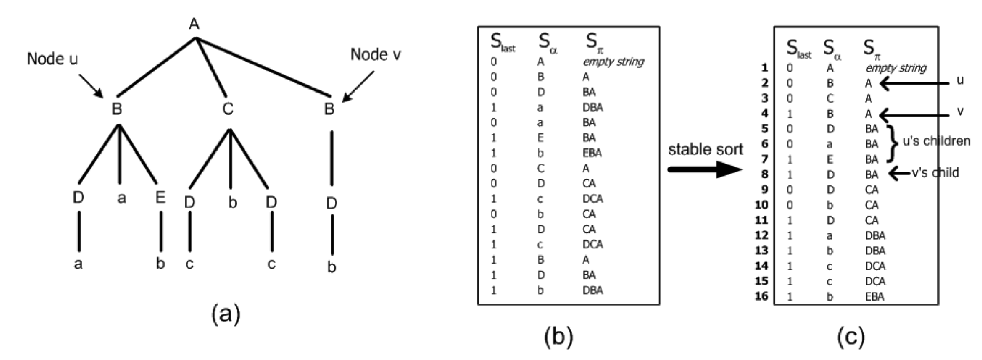
\includegraphics[width=1\textwidth]{Immagini/XBWT_example.png}
    \caption[XBWT example]{(a) A labeled tree $T$ where $\Sigma_N = \{A, B, C, D, E\}$ and $\Sigma_L = \{a, b, c\}$. Notice that $\alpha[u] = \alpha[v] = B$ and $\pi[u] = \pi[v] = A$. (b) The multi-set $S$ is obtained after the pre-order visit of $T$. (c) The final multi-set $S$ after the stable sort based on the $\pi$'s component of its triplets.}
    \label{fig:XBWT_example}
\end{figure}
\end{comment}


\begin{comment}
\alessio{Maybe all of this detail is not required for this algorithm... This is just a precursor of the {\pathsort}, which you explain in detail just after this subsubsection. Here, I think it's enough to give an intuition of the mod 3 stuff, and explain directly the {\pathsort}. Otherwise it can be confusing as you were talking about compressing trees and you jump to strings. I won't delete what you wrote because there are some comments that are still interesting (old part between the horizontal lines).}

\par\noindent\rule{\textwidth}{0.4pt}
Let us see briefly how the Skew algorithm works first.

\subsubsection{Skew Algorithm}
The Skew algorithm is an efficient method for constructing the suffix array of a string in linear time. A suffix array is a data structure that lists the starting indices of all the suffixes of a string in lexicographical order, and it is widely used in various string processing algorithms.

\paragraph{Step 0: Construct a Sample.}
For $k \in \{0,1,2\}$, define the index sets
\[
B_k = \{ i \in [0, n] \mid i \bmod 3 = k \}. 
\]
\alessio{If 0 and n are included, then it should be [1, n], otherwise you are counting n+1 elements. Moreover, in the XBWT table, the index starts at 1. Just checked the paper, they also consider the end character but don't represent it. I think that starting at 1 is ok then.}
Let $C = B_1 \cup B_2$ be the set of sample positions, and let $S_C$ denote the set of sample suffixes. \alessio{What does sample mean? Suffixes of what? What is the formal definition of $S_C$?}

\paragraph{Step 1: Sort Sample Suffixes.}
For both $k = 1$ and $k = 2$, construct the string $R_k$ whose characters are the triples $[t_i, t_{i+1}, t_{i+2}]$ for $i \in B_k$, in increasing order. \alessio{What are the $t_i$s? Also, the original paper uses a different notation with $k$ as subscript that is slightly clearer. Show how $R$ is made $[ttt][ttt]...$}
The last character of $R_k$ is unique because we pad it with sentinels so that $t_{n+1} = t_{n+2} = 0$. Let $R = R_1 R_2$ be the concatenation of $R_1$ and $R_2$.
Then the non-empty suffixes of $R$ correspond to the sample suffixes in $S_C$ in an order-preserving way: sorting the suffixes of $R$ yields the order of $S_C$.
To sort the suffixes of $R$, first radix sort the characters of $R$ (the triples) and rename them by their ranks to obtain a string $R'$. If all characters are distinct, their order directly gives the order of suffixes. Otherwise, sort the suffixes of $R'$ recursively using the same DC3 procedure.
Once $S_C$ is sorted, assign ranks to sample suffixes: for $i \in C$, let $\mathrm{rank}(S_i)$ be the rank of $S_i$ within $S_C$. Additionally, define $\mathrm{rank}(S_{n+1}) = \mathrm{rank}(S_{n+2}) = 0$. For $i \in B_0$, $\mathrm{rank}(S_i)$ is undefined.
\alessio{This paragraph is very complicated. The previous version (which Nicola didn't comment much on) was much clearer, despite being less formal. In particular: you don't define what sample means, what is $t_i$ in the triplets, what is $S_C$ and how it correlates to $R$, how the renaming works, what are the ranks of the triplets, what is the DC3 procedure. I can see that you copied the explanation of the original paper to be consistent with their notation, but you should be consistent with \textbf{your} notation. For example: you defined strings with $S = ...s_i...$ but here you use $t$. But $T$ in your thesis is a tree and you want to build a tree, so it seems like you are creating triplets of nodes of the tree.}
\alessio{Also, an example would help a lot (you can copy the one of the original paper if you want).}

\paragraph{Step 2: Sort Non-sample Suffixes.}
Represent each non-sample suffix $S_i$ with $i \in B_0$ using the pair
\[
\bigl(t_i,\ \mathrm{rank}(S_{i+1})\bigr).
\]
Note that $\mathrm{rank}(S_{i+1})$ is always defined for $i \in B_0$ by the previous step. Then, radix sort these pairs to obtain the order of $S_{B_0}$.

\paragraph{Step 3: Merge.}
Merge the two sorted sets $S_C$ and $S_{B_0}$ using a standard comparison-based merging. To compare a suffix $S_i \in S_C$ against a suffix $S_j \in S_{B_0}$, distinguish two cases:
\[
\begin{aligned}
&\text{if } i \in B_1: && S_i \le S_j \iff \bigl(t_i,\ \mathrm{rank}(S_{i+1})\bigr) \le_{\mathrm{lex}} \bigl(t_j,\ \mathrm{rank}(S_{j+1})\bigr),\\
&\text{if } i \in B_2: && S_i \le S_j \iff \bigl(t_i,\ t_{i+1},\ \mathrm{rank}(S_{i+2})\bigr) \le_{\mathrm{lex}} \bigl(t_j,\ t_{j+1},\ \mathrm{rank}(S_{j+2})\bigr).
\end{aligned}
\]
The ranks used above are defined in all cases by Step~1. Each comparison inspects $O(1)$ characters/ranks, and the two-way merge advances each pointer at most once, so the merge runs in linear time overall.

\paragraph{Time Complexity.}
Excluding the recursive call, all steps are linear-time via radix sorting and a single-pass merge. The recursion operates on a string of length $2n/3$, so the overall time satisfies
\[
T(n) \;=\; T(2n/3) + O(n) \;=\; O(n).
\]

\par\noindent\rule{\textwidth}{0.4pt}
\end{comment}

% \subsubsection{PathSort Algorithm} \label{sec:pathSort}

% The pseudocode of the pathSort algorithm is shown in \cref{alg:pathSort}. 
The {\pathsort} algorithm works similarly, adapted to work on labeled trees.
% This algorithm is based on the Skew algorithm, but it is adapted to work on labeled trees.
\alessio{What is an upward subpath? Is it the $\pi$ component of the node or is it something with the triplets? If it is the first case, use $\pi(u)$, otherwise define upward subpath. Reading the Ferragina et al paper it seems $\pi$ (or at least, some prefix), so i will edit it. The original version is in the old stuff folder.}
Given a value $j\in\{0,1,2\}$, the main idea is to recursively sort the $\pi$ component of the nodes in levels $\not\equiv j \pmod{3}$, then sort the $\pi$ component of the nodes in levels $\equiv j \pmod{3}$ using the result of the previous step, and finally merge the resulting two sets. %by exploiting their lexicographic names.
At each step $i$ of the recursion, the algorithm works on a labeled tree $T_i$, which is a \emph{contracted} (or shrunk) version of the original tree $T$. 
We set $T_0 = T$, and note that the structure of $T_{i+1}$ is derived from that one of $T_i$.
The inner workings of the recursive step will be explained in detail later.

The parameter $j$ is chosen in such a way that the number of nodes of the shrunk tree whose level is $\equiv j \pmod{3}$ is at least $t/3$, so that a constant fraction of upward paths $\pi$ is ensured to be dropped at each recursive step.
It is important to note that:
\begin{enumerate}
    \item the height of the new (contracted) tree shrinks by a factor of three, hence the node naming requires the radix sort over triples of names; 
    \item given the choice of $j$, the number of nodes of the new (contracted) tree will be at most $2t/3$, thus ensuring that the running time of the algorithm satisfies the recurrence $R(t) = R(2t/3) + \Theta(t) = \Theta(t)$; 
    \item following an argument similar to~\cite{karkkainen2006linear}, the names of the dropped subpaths can be computed in $O(t)$ time from the names of the non-dropped subpaths, by radix sorting.
\end{enumerate}
The pseudocode of the {\pathsort} algorithm is shown in \cref{alg:pathSort}.

\begin{algorithm}
    \caption{{\pathsort}($T$)}
    \label{alg:pathSort}
    \begin{algorithmic}[1]
    \State Initialize the array of triplets \texttt{IntNodes}[1 \dots $t$].
    \State Visit the internal nodes of $T$ in pre-order. For the $i$-th visited internal node $u$, set $\texttt{IntNodes}[i] = \bigl(\alpha(u),\, \text{level}(u),\, \text{parent}(u)\bigr)$.
    \State Let $j \in \{0, 1, 2\}$ be such that the number of nodes in \texttt{IntNodes} whose level is $\equiv j \pmod{3}$ is at least $t/3$. Sort recursively the upward subpaths starting at nodes in levels $\not\equiv j \pmod{3}$.
    \State Sort the upward subpaths starting at nodes in levels $\equiv j \pmod{3}$ using the result of Step 3.
    \State Merge the two sets of sorted subpaths by exploiting their lexicographic names.
    \end{algorithmic}
\end{algorithm}

\subsubsection{Recursive Step of PathSort}
At each recursive step, the algorithm constructs the array \texttt{IntNodes}, which stores the triplets $(\alpha(u), \text{level}(u), \text{parent}(u))$ for every internal node $u$ in the given tree $T$.  

Next, the algorithm selects a value $j$ such that the number of nodes in \texttt{IntNodes} with depth $\equiv j \pmod{3}$ is at least $t/3$. Based on this choice, two separate arrays are created:  
\begin{itemize}
    \item \texttt{IntNodesAtPosJ}, containing nodes at levels $\equiv j \pmod{3}$,
    \item \texttt{IntNodesNotAtPosJ}, containing nodes at levels $\not\equiv j \pmod{3}$
\end{itemize}

For each node $u$ in \texttt{IntNodesNotAtPosJ}, the algorithm extracts the upward path consisting of the first three ancestors of $u$, $\pi(u)[1 \dots 3]$. These paths are then sorted using radix sort. If all upward paths are unique, the nodes in \texttt{IntNodesAtPosJ} are sorted and subsequently merged with \texttt{IntNodesNotAtPosJ} using lexicographic ordering.
%, following the same merging strategy as in the Skew algorithm. 
Otherwise, the algorithm recursively calls the {\pathsort} function on a new contracted tree, where nodes are renamed according to their sorted paths.

\subsection{Inversion}
The ability to invert the XBWT is fundamental to its utility as a compression technique. Invertibility guarantees that the original tree can be perfectly reconstructed from its transformed representation ($S_{\text{last}}$ and $S_{\alpha}$). This ensures that the compression is lossless, meaning that no information is lost during the process, which is a critical requirement for most applications.

The property `Path-based Indexing' (\cref{prop3}) ensures that the two arrays $S_{\text{last}}$ and $S_{\alpha}$ of the XBWT can be used to reconstruct the original tree $T$. The algorithm for inverting the XBWT is linear in time and requires $O(t \log t)$ bits of space.

\cref{alg:rebuildTree} operates in three main steps. First, it constructs two auxiliary arrays, $F$ and $J$, which are crucial for navigating the tree structure within the compressed format.

\begin{itemize}
    \item \textbf{The $F$ array:} This array maps each character $c \in \Sigma$ to the index of the first occurrence in $S$ of a triplet whose $\pi$-component is prefixed by $c$. It essentially marks the starting points of blocks of nodes that share the same initial path label.
    \item \textbf{The $J$ array:} For each entry $i$ in $S$, $J[i]$ stores the index in $S$ corresponding to the first child of the node represented by $S[i]$. If $S[i]$ represents a leaf, $J[i]$ is set to a sentinel value (e.g., -1).
\end{itemize}

\begin{example}[$F$ and $J$ arrays]
    Considering the XBWT in \cref{tab:xbwt_example}, the $F$ array would map 'A' to index 2 (for node $r$), 'B' to index 5 (for the children of nodes with label 'B'), and so on. For the $J$ array, let's take the node $u$ at index 2 in $S$. Its first child is at index 5. Therefore, $J[2]$ would be 5.
\end{example}

Finally, the algorithm employs the array $J$ to
simulate a depth-first visit of $T$, creates its labeled nodes, and properly connects them to their parents. 

% \alessio{Why BuildF and BuildJ take in input XBWT[T] but do not use it? The function should use the parameters that you pass it, pass more specific variables (as below). Also, I removed XBWT[T] notation since I really don't like it :).}
\begin{algorithm}[H]
    \caption{\textsc{RebuildTree}($S_\alpha$, $S_\textup{last}$)}
    \label{alg:rebuildTree}
    \begin{algorithmic}[1]
    \State $F = $ \textsc{BuildF}($S_\alpha$, $\Slast$)
    \State $J = $ \textsc{BuildJ}($S_\alpha$, $\Slast$, $F$)
    \State Create node $r$ and set $Q = \{\langle1, r\rangle\}$; \Comment{$Q$ is a stack}
    \While{$Q \neq \emptyset$} \Comment{We still have nodes to create in $T$}
        \State $\langle i, u \rangle = $ pop($Q$);
        \State $j = J[i]$; \Comment{Take the block of $u$'s children in $S$}
        \If{$j = -1$} \Comment{$u$ is a leaf of $T$}
            \State \textbf{continue};
        \EndIf
        \State Find first $j' \geq j$ such that $S_{\text{last}}[j'] = 1$; \Comment{Range $[j, j']$ are the children of $u$ in $T$}
        \For{$h = j'$ downto $j$} 
            \State Create the node $v$ labeled $S_\alpha[h]$;
            \State Attach $v$ as first child of $u$;
            \State push($\langle h, v \rangle$, $Q$);
        \EndFor
    \EndWhile
    \State \Return node $r$.
    \end{algorithmic}
\end{algorithm}

\begin{algorithm}[H]
    \caption{\textsc{BuildF}($S_\alpha$, $\Slast$)}
    \label{alg:buildF}
    \begin{algorithmic}[1]
    \State $C[1,|\Sigma_n|] = \{0, 0, \dots, 0\}$;
    \State $F[1,t] = \{0, 0, \dots, 0\}$;
    \For{$i = 1, \ldots, t$}
        \State $C[S_\alpha[i]] = C[S_\alpha[i]] + 1$; \Comment{Count the occurrences of node labels}
    \EndFor
    \State $F[1] = 2$; \Comment{$S_\pi[1]$ is the empty string}
    \For{$i \in \{1, \ldots, |\Sigma_N|-1\}$} \Comment{Consider just the internal-node labels}
        \State $s = 0$; $j = F[i]$;
        \While{$s \neq C[i]$} \Comment{Not all blocks of children have been passed}
            \State $j = j + 1$;
            \If{$S_{\text{last}}[j] = 1$} \Comment{One further block of children has passed}
                \State $s = s + 1$;
            \EndIf
        \EndWhile
        \State $F[i+1] = j$;
    \EndFor
    \State \Return $F$.
    \end{algorithmic}
\end{algorithm}
    
\begin{algorithm}[H]
    \caption{\textsc{BuildJ}($S_\alpha$, $\Slast$, $F$)}
    \begin{algorithmic}[1]
    \State $J[1,t]=\{0, 0, \dots, 0\}$;
    \For{$i = 1, \ldots, t$}
        \If{$S_\alpha[i] \in \Sigma_L$}
            \State $J[i] = -1$; \Comment{$S_\alpha[i]$ is a leaf label}
        \Else
            \State $J[i] = F[S_\alpha[i]]$;
            \State $z = J[i]$;
            \While{$S_{\text{last}}[z] \neq 1$} \Comment{Reach the last child of $S_\alpha[i]$}
                \State $z = z + 1$;
            \EndWhile
            \State $F[S_\alpha[i]] = z + 1$;
        \EndIf
    \EndFor
    \State \Return $J$.
    \end{algorithmic}
\end{algorithm}

\subsection{Compressing Labeled Trees}
\begin{comment}
Let the $k$-context of a node $u \in T$ be the first $k$ symbols of $\pi(u)$. We denote this $k$-long prefix as $\pi_k[u]$. Thus, $\pi_k[u]$ represents the subpath of length $k$ leading to $u$ in $T$, or equivalently, the node $u$ descends from a subpath labeled as $\pi_k[u]$, where the nodes in $\pi_k[u]$ are encountered in an upward direction.
\end{comment}

The XBWT of a tree $T$ exhibits a local homogeneity property on $S_{\alpha}$: the labels ($\alpha$ components) of nodes whose upward paths ($\pi$ components) share long common prefixes appear in $S_{\alpha}$ in contiguous (or tightly bounded) clusters. 
This phenomenon can be formalized via the notion of $k$-contexts on trees.
This property mirrors the strong local homogeneity exhibited by strings under the Burrows-Wheeler Transform~\cite{burrows1994block} when applied to labeled trees.

To illustrate this, let us consider two arbitrary nodes $u$ and $v$ in $T$, and examine their contexts $\pi(u)$ and $\pi(v)$. Given the sorting of $S$, the greater the length of the shared prefix between $\pi(u)$ and $\pi(v)$, the closer the corresponding labels $\alpha(u)$ and $\alpha(v)$ will be in the string $S_{\alpha}$. These closely spaced labels are expected to be few in number, resulting in $S_{\alpha}$ exhibiting local homogeneity. As a consequence, we can leverage the advanced algorithmic techniques developed for BWT-based compression methods to achieve efficient compression.

At the end, the XBWT is used for turning the labeled tree compression problem into a string compression problem. To this aim, two string compressors
$C_{\alpha}$ and $C_{\text{last}}$ are used to compress the two strings $S_{\alpha}$ and $S_{\text{last}}$. respectively, by exploiting their fine specialties. Of course, many choices are possible for $C_{\alpha}$ and $C_{\text{last}}$, each having implications on the algorithmic time and compression bounds.

In general, the following theorem holds:

\begin{theorem}[\cite{ferragina2009compressing}, Theorem 4]
    let $C_{\alpha}$ be a $k$-th order string compressor that compresses any string $w$ into $|w|H_k(w) + |w| + o(|w|)$ bits, taking $O(|w|)$ time; and let $C_{\text{last}}$ be an algorithm that stores $S_{\text{last}}$ without compression. With this simple instantiation, the labeled tree $T$ can be compressed within $t H_k(S_{\alpha}) + 2t + o(t)$ bits and takes $O(t)$ optimal time.
\end{theorem}

Since $H_k(S_\alpha) \leq (\log |\Sigma|) + 1$
(where the additional $+1$ cost comes from the definition of $\alpha$ in \cref{def:node_informations}, since we consider the same alphabet $\Sigma$ for nodes and leaves), the above bound is at most $t(\log |\Sigma| + 3) + o(t)$ bits, and can be significantly better than the information-theoretic lower bound and the plain storage of the XBWT (both taking $2t + t \log|\Sigma|$ bits), depending on the distribution of the labels among its nodes.

\subsection{Indexing a Compressed Labeled Tree} \label{sec:xbwt_operations}
In order to implement the efficient operations listed in \cref{compandindexinglabtree} using the compressed arrays $S_{\text{last}}$ and $S_{\alpha}$ of XBWT, we need the chosen compressors $C_{\alpha}$ and $C_{\text{last}}$ to support the following operations:

Given a string $S[1, t]$ over alphabet $\Sigma$
\begin{itemize}
    \item \textbf{$rank_c(S, q)$}: gives the number of times the symbol $c \in \Sigma$ appears in $S[1, q]$.
    \item \textbf{$select_c(S, i)$}: gives the position of the $i$-th occurrence of the symbol $c \in \Sigma$ in $S$.
\end{itemize}

The compressed indexing of the XBWT will be based on three compressed data structures that support rank and select queries over the two strings $S_{\alpha}$ and $S_{\text{last}}$, and over an auxiliary binary array $A[1, t]$ defined as: $A[1] = 0$, $A[j] = 1$ if and only if the first symbol of $S_{\pi}[j]$ differs from the first symbol of $S_{\pi}[j - 1]$. 
Hence, $A$ contains at most $|\Sigma| + 1$ bits set to 1 out of $t$ positions. It is also easy to see that, through rank and select operations over $A$, we can succinctly implement the array $F$ employed in \cref{alg:rebuildTree,alg:buildF}.

%\alessio{Is $S$ a pair of strings or a string of pairs? $S$ such that $S[i] = (\Slast[i], S_\alpha[i])$, for $i = 1,...,t$?}
In this section, let $S \coloneq (S_{\text{last}}, S_{\alpha})$ such that $S[i] = (\Slast[i], S_\alpha[i])$ for $i = 1,\dots,t$, denote the XBWT obtained after the construction phase.
The compressed index supports the following methods:

\textbf{GetRankedChild($i$, $k$)}: Returns the position in $S$ of the $k$-th child of the node at index $i$. If the child does not exist, it returns -1. 
\begin{example}
    In \cref{tab:xbwt_example_2}, \texttt{GetRankedChild(2, 2)} returns 6.
\end{example}

\textbf{GetCharRankedChild($i$, $c$, $k$)}: Returns the position in $S$ of the $k$-th child labeled $c$ of the node at index $i$. If the child does not exist, it returns -1.
\begin{example}
    In \cref{tab:xbwt_example_2}, \texttt{GetCharRankedChild(1, B, 2)} returns 4.
\end{example}

\textbf{GetDegree($i$)}: Returns the total number of children of the node at index $i$ in $S$.

\textbf{GetCharDegree($i$, $c$)}: Returns the number of children of the node at index $i$ in $S$ that have the label $c$.

\textbf{GetParent($i$)}: Returns the position in $S$ of the parent of the node at index $i$. If the node is the root (at index 1), it returns -1.
\begin{example}
    In \cref{tab:xbwt_example_2}, \texttt{GetParent(8)} returns 4.
\end{example}

\textbf{GetSubtree($i$)}: Retrieves the labels of all nodes in the subtree rooted at the node at index $i$ in $S$. The labels can be returned in any standard traversal order (e.g., pre-order, in-order, or post-order).

\textbf{SubPathSearch($P$)}: For a given labeled path $P = c_1c_2 \cdots c_k$, this function finds the range $[\text{First}\dots\text{Last}]$ such that all strings in $S_{\pi}[\text{First}\dots\text{Last}]$ are prefixed by the reversed path $P^R = c_k \cdots c_2c_1$.
\begin{example}
    In \cref{tab:xbwt_example_2}, \texttt{SubPathSearch(BD)} results in the range [12, 13], and \\ \texttt{SubPathSearch(AB)} gives the range [5, 8].
\end{example}

It is important to note that their time complexity is dependent on the specific implementation for rank and select over the compressed strings $S_{\alpha}$ and $S_{\text{last}}$. 

Let's now see how to implement some of the above methods (from which the others can be derived) using the rank and select operations over the compressed strings $S_{\alpha}$ and $S_{\text{last}}$.

\begin{figure}
    \centering
    \begin{tabular}{r c c c l}
    \hline\hline
    \textbf{} & $A$ & $S_{\text{last}}$ & \textbf{$S_{\alpha}$} & \textbf{$S_{\pi}$} \\
    \hline
    \textbf{1} & 0 & 0 & A & $\epsilon$ \\
    \textbf{2} & 1 & 0 & B & A \\
    \textbf{3} & 0 & 0 & C & A \\
    \textbf{4} & 0 & 1 & B & A \\
    \textbf{5} & 1 & 0 & D & BA \\
    \textbf{6} & 0 & 0 & a & BA \\
    \textbf{7} & 0 & 1 & E & BA \\
    \textbf{8} & 0 & 1 & D & BA \\
    \textbf{9} & 1 & 0 & D & CA \\
    \textbf{10} & 0 & 0 & b & CA \\
    \textbf{11} & 0 & 1 & D & CA \\
    \textbf{12} & 1 & 1 & a & DBA \\
    \textbf{13} & 0 & 1 & b & DBA \\
    \textbf{14} & 0 & 1 & c & DCA \\
    \textbf{15} & 0 & 1 & c & DCA \\
    \textbf{16} & 1 & 1 & b & EBA \\
    \hline\hline
    \end{tabular}
    \caption{The sequence $S$ for the tree shown in \cref{fig:example_tree}, obtained by stably sorting triplets according to their `$\pi$' components. In contrast to \cref{tab:xbwt_example}, the auxiliary binary array $A$ is shown in the second column.}
    \label{tab:xbwt_example_2}
\end{figure}

\subsubsection*{GetChildren($i$)}
\cref{alg:getchildren} exploits directly the properties described before, in particular Property `Path-based Indexing' (\cref{prop3}). The rank operation at line 5 is used to get the number $r$ of nodes labeled $c$ up to position $i$ in $S_{\alpha}$. Then, the position $F[c]$ is obtained through a select operation on $A$ (line 6). By Property `Path-based Indexing', the children of $S[i]$ are located at the $r$-th block of children following position $F[c]$. Lines $8 - 9$ identify this block. 

\begin{example}
    Let's walk through an example using \cref{tab:xbwt_example_2}. Consider the node $u$ at index 2 labeled with $B$. To find its children:

    \begin{enumerate}
        \item First, we compute $r = 1$ since this is the first occurrence of $B$ in $S_{\alpha}$ up to position 2.
        \item Next, we find $y = F[B] = 5$, which marks the start of the block containing children of all nodes labeled $B$.
        \item Then, we count $z = 1$ ones in $S_{\text{last}}$ up to position $y-1$.
        \item Finally, the children block is delimited by the $z+r-1 = 1$st and $z+r = 2$nd ones in $S_{\text{last}}$, giving us the range $[5,7]$.
    \end{enumerate}

    This range $[5,7]$ indeed contains the three children of the node at index 2, as we can verify from the tree structure in \cref{fig:example_tree}.
\end{example}

\begin{algorithm}[H] 
    \caption{GetChildren($S_\alpha$, $\Slast$, $i$)}
    \label{alg:getchildren}
    \begin{algorithmic}[1]
    \If{$S_\alpha[i] \in \Sigma_L$}
        \State \Return $-1$ \Comment{$S[i]$ is a leaf}
    \EndIf
    \State $c = S_\alpha[i]$ \Comment{$S[i]$ is labeled $c$}
    \State $r = \text{rank}_c(S_\alpha, i)$
    \State $y = \text{select}_1(A, c)$ \Comment{$y = F[c]$}
    \State $z = \text{rank}_1(S_{\text{last}}, y - 1)$
    \State $\text{First} = \text{select}_1(S_{\text{last}}, z + r - 1) + 1$
    \State $\text{Last} = \text{select}_1(S_{\text{last}}, z + r)$
    \State \Return $(\text{First}, \text{Last})$
    \end{algorithmic}
\end{algorithm}

\subsubsection*{GetParent($i$)}
\cref{alg:getparent} is based on Property `Path-based Indexing' (\cref{prop3}) and it is the inverse of the GetChildren method. In line 4, the algorithm computes the label $c$ of the parent of $S[i]$ that prefixes the upward path leading to $S[i]$. Then, the parent of $S[i]$ is searched among the nodes labeled $c$ in $S_{\alpha}$ by exploiting Property `Path-based Indexing' in a reverse manner. Namely, the number $k$ of children-blocks in the range $S[y, i]$ is computed; these are children of nodes labeled $c$ and preceding $i$ in the stable sort of $S$. Then, the $k$-th occurrence of $c$ in $S_{\alpha}$ is selected, which is indeed the parent of $S[i]$.

\begin{example}
    Let's illustrate how to find a node's parent using \cref{tab:xbwt_example_2}. Consider node $v$ located at index 4 with label $B$. The process to find its parent involves:
    \begin{enumerate}
        \item Computing $c = \text{rank}_1(A, 4) = 1$, which tells us the parent has label `A' (as $A$ contains exactly one 1 up to position 4).
        \item Locating $y = F[A] = 2$, which indicates where the block of children for nodes labeled `A' begins.
        \item Calculating $k = \text{rank}_1(S_{\text{last}}, 4-1) - \text{rank}_1(S_{\text{last}}, 2-1) = 0$, meaning no complete child blocks appear before position 4.
        \item Therefore, $v$'s parent is the first ($(k+1)$-th) occurrence of `A' in $S_{\alpha}$, corresponding to index 1 (the root of $\mathcal{T}$).
    \end{enumerate}
    This example demonstrates how the XBWT structure efficiently encodes parent-child relationships using just the $S_{\text{last}}$ and $S_{\alpha}$ arrays.
\end{example}

\begin{algorithm}[H]
    \caption{GetParent($S_\alpha$, $\Slast$, $i$)}
    \label{alg:getparent}
    \begin{algorithmic}[1]
    \If{$i = 1$}
        \State \Return $-1$ \Comment{$S[i]$ is the root of $\mathcal{T}$}
    \EndIf
    \State $c = \text{rank}_1(A, i)$
    \State $y = \text{select}_1(A, c)$
    \State $k = \text{rank}_1(S_{\text{last}}, i - 1) - \text{rank}_1(S_{\text{last}}, y - 1)$
    \State $p = \text{select}_c(S_\alpha, k + 1)$
    \State \Return $p$
    \end{algorithmic}
\end{algorithm}

\subsubsection*{SubPathSearch($P$)}
We assume that $P = c_1c_2 \cdots c_k$ algorithm SubPathSearch computes the range $[First, Last]$ in $|P| = l$ phases, each one preserving the following invariant:

\begin{itemize}
    \item Invariant of Phase $i$. At the end of the phase, $S_{\pi}[First]$ is the first entry prefixed by $P[1, i]^R$ , and $S_{\pi}[Last]$ is the last entry prefixed by $P[1, i]^R$ , where $s^R$ is the reversal of string $s$.
\end{itemize}

At the beginning (i.e., $i = 1$), First and Last are easily determined via the entries $F[c_1]$ and $F[c_1 + 1] - 1$, which point to the first and last entry of $S_{\pi}$ prefixed by $c_1$ (by definition of array $F$). Since we do not have the $F$ array, we implement these operations via rank and select queries over array $A$. Let us assume that the invariant holds for Phase $i - 1$, and prove that the $i$-th iteration of the for-loop in algorithm SubPathSearch preserves the invariant. More precisely, let $S_{\pi}[First, Last]$ be all entries prefixed by $P[1, i - 1]^R$. So $S[First, Last]$ contains all nodes descending from $P[1, i - 1]$. SubPathSearch determines $S[z_1]$ (respectively $S[z_2]$) as the first (respectively last) node in $S[First, Last]$ that descends from $P[1, i - 1]$ and is labeled $c_i$, if any. Then it jumps to the first child of $S[z_1]$ and the last child of $S[z_2]$. From Property 2 (item 2) and the correctness of algorithms GetChildren and GetDegree, we infer that the positions of these two children are exactly the first (respectively last) entry in $S$ whose $\pi$-component is prefixed by $P[1, i]^R$. 

The time complexity of the SubPathSearch algorithm is $O(l)$, where $l$ is the length of the input path $P$.

\begin{example}
    Consider the tree in \cref{fig:example_tree}, and let $P = BD$. The algorithm \textsc{SubPathSearch}($P$) returns the range $[12, 13]$ through the following steps:

    \begin{enumerate}
        \item Initially, $First = F[B] = 5$ and $Last = F[C] - 1 = 8$. The range $S[5,8]$ contains all nodes descending from paths prefixed by $B$.
        
        \item For $c_2 = D$:
        \begin{itemize}
            \item Compute $k_1 = 0$ and $k_2 = 2$
            \item This yields $z_1 = 5$ and $z_2 = 8$
            \item The first child of $S[5]$ is at position $12$
            \item The last (and only) child of $S[8]$ is at position $13$
        \end{itemize}
        
        \item Therefore, the algorithm returns the range $[12,13]$
    \end{enumerate}

    Note that the number of occurrences of subpath $P$ is 2, as evidenced by the two occurrences of 1 in range $S_{\text{last}}[12,13]$.
\end{example}

\begin{algorithm}[H]
    \caption{\textsc{SubPathSearch}($S_\alpha$, $\Slast$, $P$)}
    \label{alg:subpathsearch}
    \begin{algorithmic}[1]
    \State $First = F(c_1)$; $Last = F(c_1 + 1) - 1$
    \If{$First > Last$}
        \State \textbf{return} ``$P$ is not a subpath of $T$''
    \EndIf
    \For{$i = 2, \dots, k$}
        \State $k_1 = \text{rank}_{c_i}(S_\alpha, First - 1)$; 
        \State $z_1 = \text{select}_{c_i}(S_\alpha, k_1 + 1)$
        \Comment{first entry in $S_\alpha[First, t]$ labeled $c_i$}
        \State $k_2 = \text{rank}_{c_i}(S_\alpha, Last)$; 
        \State $z_2 = \text{select}_{c_i}(S_\alpha, k_2)$
        \Comment{last entry in $S_\alpha[1, Last]$ labeled $c_i$}
        \If{$z_1 > z_2$}
            \State \textbf{return} ``$P$ is not a subpath of $T$''
        \EndIf
        \State $First = \text{GetRankedChild}(z_1, 1)$ \Comment{get the first child of $S[z_1]$}
        \State $Last = \text{GetRankedChild}(z_2, \text{GetDegree}(z_2))$ \Comment{get the last child of $S[z_2]$}
    \EndFor
    \State \textbf{return} $(First, Last)$
    \end{algorithmic}
\end{algorithm}

\subsection{Summary}
To sum up, the XBWT has several key properties that make it an effective tool for labeled tree compression and indexing:
\begin{itemize}
    \item \textbf{Succinctness:} The XBWT representation of a labeled tree uses space close to the worst-case entropy (\cref{lem:info_theoretic_lower_bound}), which is \(H_{wc} = 2t + t \log |\Sigma| - \Theta(\log t) \) bits for a tree with $t$ nodes and an alphabet of size $|\Sigma|$.
    Notice that the second component of $H_{wc}$ is $t\log |\Sigma|$ and not $m\log |\Sigma|$ since the XBWT works on \emph{node} labeled trees.
    \item \textbf{Efficient Querying:} The XBWT supports navigational queries (\cref{def:tree_operations}) in optimal time $O(1)$ if $|\Sigma| = O(polylog(t))$, otherwise in $O(\log\log^{1+\epsilon} |\Sigma|)$ time. Whereas, given $s \in \Sigma^*$, subpath queries (\cref{def:tree_operations}) are supported in $O(|s|)$ if $|\Sigma| = O(polylog(t))$, otherwise in $O(|s| \log\log^{1+\epsilon} |\Sigma|)$ time.
    \item \textbf{Scalability:} The XBWT is particularly useful for large-scale hierarchical data, such as XML documents or phylogenetic trees, where both compression and fast querying are critical.
\end{itemize}